\section{The VAMPIRES instrument}\label{sec:design}

\begin{figure*}[t]
    \centering
    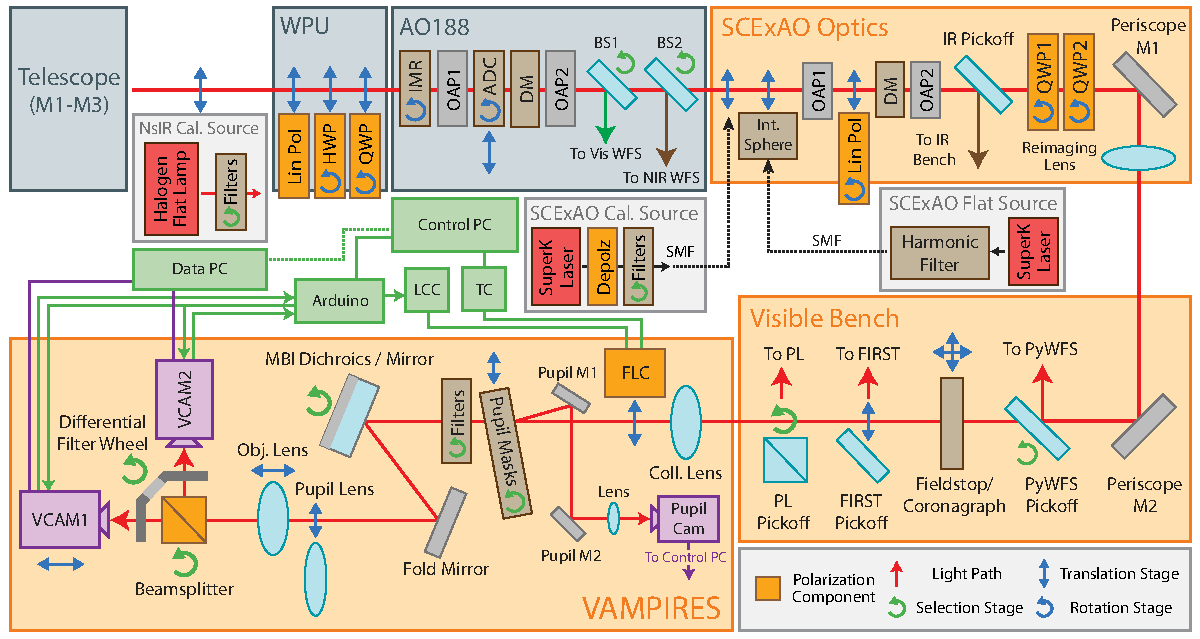
\includegraphics[width=\textwidth]{figures/VAMPIRES_diagram.pdf}
    \caption{VAMPIRES Instrument Schematic including all common path instruments: the telescope, waveplate unit (WPU), AO188, and SCExAO. Some components are simplified or omitted for clarity and are not to scale. NsIR: Nasymth infrared platform of the Subaru telescope, HWP: half-wave plate, QWP: quarter-wave plate, IMR: image rotator (k-mirror), OAP: off-axis parabolic mirror, ADC: atmospheric dispersion corrector, DM: deformable mirror, BS: beamsplitter, PyWFS: pyramid wavefront sensor, PL: photonic lantern, SMF: single-mode fiber, FLC: ferroelectric liquid crystal, LCC: liquid-crystal controller, TC: temperature controller, ND: neutral density filter.}
    \label{fig:schematic}
\end{figure*}

The Visible Aperture-Masking Polarimetric Imager/Interferometer for Resolving Exoplanetary Signatures (VAMPIRES) is the visible-light (\SIrange{600}{775}{\nano\meter}) sub-instrument of the Subaru Coronagraphic Extreme Adaptive Optics testbed (SCExAO; \citealp{jovanovic_subaru_2015}). SCExAO is a platform for high-contrast imaging and technology development on the \SI{8.2}{\meter} Subaru telescope; the multi-stage adaptive optics achieves diffraction-limited imaging at visible wavelengths, and the large telescope diameter produces angular resolutions of $\sim$\SI{20}{\mas}. Observing modes and science use cases for VAMPIRES are detailed in \autoref{tbl:modes}.

\begin{deluxetable*}{p{1.2in}p{2.5in}p{3in}}
\tabletypesize{\small}
\tablehead{
    \colhead{Mode} & 
    \colhead{Description} &
    \colhead{Use Cases}
}
\tablecaption{VAMPIRES observing configurations.\label{tbl:modes}}
\startdata
\multicolumn{3}{l}{\textit{Filters}} \\
Standard & Open, 625-50, 675-50, 725-50, 750-50, 775-50 & Highest throughput with Open filter \\
Multiband & F620, F670, F720, F760 & Spectral differential imaging, color analysis, phase diversity \\
Narrowband & H$\alpha$, H$\alpha$-Cont, SII, SII-Cont & Narrowband spectral differential imaging, accreting protoplanets, stellar jets, stellar atmospheres \\
\hline \multicolumn{3}{l}{\textit{Polarimetry}} \\
% \cutinhead{Polarimetry}
Fast polarimetry & Triple-difference with HWP+FLC\newline (DIT$<$\SI{1}{\second}) & Circumstellar disks, sub-stellar companions, stellar atmospheres, stellar jets, solar system objects \\
Slow polarimetry & Double-difference with HWP & Circumstellar disks, stellar jets, solar system objects \\
\hline \multicolumn{3}{l}{\textit{Coronagraphy}} \\
No coronagraph & 5$\sigma$ contrast: $10^{\text{-}3}$ at \ang{;;0.1}, $10^{\text{-}4}$ at $>$\ang{;;0.4} & Stellar companions, circumstellar disks (with PDI), solar system objects \\
Classic Lyot & IWA: 37, 59, 105, or 150 \si{\mas};\newline 5$\sigma$ contrast: $10^{\text{-}4}$ at \ang{;;0.1}, $10^{\text{-}6}$ at $>$\ang{;;0.5} & Sub-stellar companions and circumstellar disks \\
Vector vortex & IWA: 61 \si{\mas}; 5$\sigma$ contrast: TBD\newline (not compatible with polarimetry) & Sub-stellar companions and circumstellar disks \\
\hline \multicolumn{3}{l}{\textit{Aperture masking}} \\
NRM interferometry & 7, 9, and 18-hole non-redundant masks, plus annulus mask (not compatible with coronagraphs) & Dust shells, stellar atmospheres, circumstellar disks \\
Redundant apodizing pupil & \ang{;;0.1} to \ang{;;0.8} dark hole resilient to $\sim$\SI{1}{\radian} of low-wind effect (not compatible with coronagraphs) & Circumstellar disks and sub-stellar companions \\
\enddata
\end{deluxetable*}


\subsection{Telescope and Common Path Instruments}

SCExAO is mounted on one of the Nasymth platforms of the Subaru telescope. The first common-path instrument is the facility waveplate unit (WPU; \citealp{watanabe_near-infrared_2018}). The WPU includes a linear polarizer, rotatable half-wave plate (HWP), and rotatable quarter-wave plate (QWP), which is used for polarimetric modulation and calibration (\autoref{sec:polarimetry}). Next is the facility AO instrument (AO188; \citealp{minowa_performance_2010}), which includes a broadband atmospheric dispersion corrector (ADC), low-order (188-element) wavefront sensor (WFS), and deformable mirror (DM). A \SI{600}{\nano\meter} longpass dichroic splits light between the WFS and downstream instruments.

\subsection{SCExAO Common Path}

Light entering SCExAO is corrected with a 2000-actuator DM at up to \SI{3.6}{\kilo\hertz} speeds for extreme AO correction \citep{lozi_new_2020,ahn_scexao_2021}. The corrected beam is split with NIR light sent to a suite of sub-instruments, including CHARIS, MEC, and FastPDI \citep{groff_charis_2015,steiger_probing_2022,lozi_status_2020}, while visible light is reflected into a periscope and reimaging lens.

A portion of the light exiting the periscope is sent to the visible pyramid WFS (PyWFS; \citealp{lozi_visible_2019}). Various dichroic and gray beamsplitters are available, but the typical configuration uses an \SI{800}{\nano\meter} shortpass dichroic. The tilt angle of this dichroic ($\sim$\ang{20}) shifts the cut-off wavelength closer to $\sim$\SI{775}{\nano\meter}. Following this pickoff is a focal plane mount that hosts a \ang{;;3}x\ang{;;3} field stop and a suite of visible coronagraphs (\autoref{sec:coronagraphy}). Following the field stop are two gray beamsplitters for fiber-fed sub-instruments \citep{vievard_single-aperture_2023,vievard_photonic_2023}.

\subsection{VAMPIRES Optics}

The remaining light (\SIrange{600}{775}{\nano\meter}) is collimated into a \SI{7.06}{\milli\meter} diameter beam. This beam passes through a removable ferroelectric liquid crystal (FLC), a pupil mask wheel, and a filter wheel. The pupil wheel houses sparse aperture masks, neutral-density (ND) filters, and the coronagraphic Lyot stops. This wheel is tilted at $\sim$\ang{6} so that a separate pupil-viewing camera can image light reflected off the masks. The standard filter wheel houses five \SI{50}{\nano\meter}-wide bandpass filters for standard imaging and an empty slot for broadband observations. After the filter wheel is a baffle isolating the VAMPIRES fore-optics.

Next, the beam reaches the multiband imaging optics and the VAMPIRES objective lens. A pupil-imaging lens can be inserted with a flip mount. As the beam converges, it passes the beamsplitter wheel, which hosts a wire-grid polarizing cube and a gray non-polarizing cube. The beamsplitters can be removed for single-camera operation. The last device before the detectors is a differential filter wheel that swaps narrowband filters between each camera for narrowband spectral differential imaging \citep{uyama_high-contrast_2020}. The two VAMPIRES detectors are described in detail in \autoref{sec:detectors}.

\subsection{Multiband Imaging} \label{sec:mbi}

One of the main goals of the VAMPIRES upgrades was enabling spectral differential imaging (SDI) without adding dispersive optics. Dispersive optics, like in an integral-field unit (IFU), require space for a prism or grating, lenslets, and reimaging optics. Space is limited in VAMPIRES to only $\sim$\SI{20}{\centi\meter} after the pupil mask. We developed a technique for ``low-resolution dispersion'' using dichroic filters to form multiple images in a compact assembly called multiband imaging (MBI).

The MBI technique is enabled by using multiple dichroics with unique angles-of-incidence (AOI) to split broadband collimated light into multiple fields imaged on the detector (\autoref{fig:mbi_schematic}). This approach takes advantage of the large sensor size of the detectors, which only uses 3\% of the detector for a \ang{;;3}x\ang{;;3} field of view (FOV)-- up to four FOVs can be tiled side-by-side before the objective lens starts to distort the off-axis images, which still only uses half the available detector area.

The optical design comprises three shortpass dichroic filters (\SI{750}{\nano\meter}, \SI{700}{\nano\meter}, and \SI{650}{\nano\meter}) plus a protected silver mirror to create four $\sim$\SI{50}{\nano\meter}-bandpass fields (\autoref{fig:filters}). The assembly can be rotated \ang{180} to become a fold mirror. A $\sim$\ang{10} protected silver fold mirror redirects the beam(s) towards the objective lens.

Ghost images are produced by repeated reflections between dichroic surfaces, which interfere with high-contrast observations. The geometry of the dichroic tilt angles was optimized so that all ghost images fall completely outside of the FOVs of the primary fields (\autoref{sec:ghosts}). Field stops are required to avoid overlap between fields, and all coronagraph masks include a field stop.

The required precision of the MBI dichroic tilt angles is on the order of $\sim$\ang{;;3} to ensure neighboring fields do not overlap. This corresponds to a linear precision of $\sim$\SI{1}{\micron} along the circumference of the \SI{25}{\milli\meter} diameter, which is $\sim$100 times finer than standard machining tolerances. Precision manufacturers NH Micro\footnote{\url{https://www.nhmicro.com/}} created titanium ring spacers and a custom lens tube using electrical-discharge machining, which has $\sim$\SI{1}{\micron} tolerances. When fully assembled, the spacers self-align in the lens tube, and interferometric analysis shows no optical distortions of the wavefront. 

\begin{figure}
    \centering
    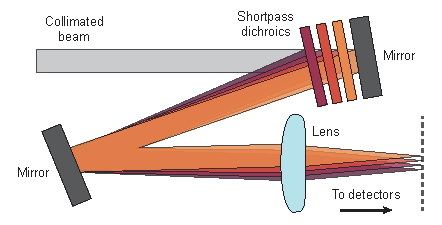
\includegraphics[width=\columnwidth]{figures/mbi_schematic.pdf}
    \caption{Schematic drawing of the multiband imaging principle. Broadband collimated light reaches the stack of tilted dichroics and mirrors. Light reflected by each dichroic creates a unique field in the focal plane due to the angle of incidence, transmitting the remaining bandpass onto the next dichroic. The final mirror reflects all remaining light through the stack.\label{fig:mbi_schematic}}
\end{figure}


% \begin{deluxetable*}{ll}
% \tabletypesize{\small}
% \tablehead{
%     \colhead{Name} & 
%     \colhead{Value(s)}
% }
% \tablecaption{VAMPIRES specifications.\label{tbl:specs}}
% \startdata
% Diff. Limit & \SI{16.5}{\mas} at \SI{625}{\nm}, \SI{20.1}{\mas} at \SI{760}{\nm}\\
% FOV & \SI{3}{\arcsecond} x \SI{3}{\arcsecond}, some cropping available \\
% F-ratio &  21.2 (28.3 in coronagraph focal plane) \\
% Pupil diameter & \SI{7.06}{\milli\meter} (1126x magnification)\\
% Min. DIT & \SI{7.2}{\micro\second} (FAST), \SI{48}{\milli\second} (SLOW) \\
% Max. framerate & \SI{500}{\hertz} (FAST), \SI{21}{\hertz} (SLOW) \\
% Coronagraph & CLC-2, CLC-3, CLC-5, CLC-7, DGVVC \\
% Pupil Masks & 7-hole, 9-hole, 18-hole, Annulus, RAP, \\
%  & LyotStop-S, LyotStop-M, LyotStop-L, \\
% & Mirror, ND1.0, ND2.5 \\
% Filters & Open, 625-50, 650-50, 675-50, 725-50, 750-50, 775-50 \\
% MBI & Dichroic stack (enabled), mirror (disabled) \\
% NB Filters & H$\alpha$, H$\alpha$-Cont, SII, SII-Cont \\
% Beamsplitter & PBS, NPBS, Open \\
% Polarimetry & Linear Stokes - HWP (modulation $>$\SI{0.5}{\second}), \\
% & Circular Stokes - QWP (modulation $>$\SI{0.5}{\second}), \\
% Pol. control & Fast FLC (modulation synced to cameras, $<$\SI{1}{\second}), \\
% & Pair of rotatable QWPs \\
% Pol. calibration & Linear polarizers, HWP, QWP \\
% \enddata
% \end{deluxetable*}
